\documentclass[12pt]{extarticle}
\usepackage[margin=1in]{geometry}
\usepackage{amsmath}
\usepackage{url}
\usepackage{color}
\usepackage{graphicx}

% my commands
\newcommand{\R}{\mathbf{R}} % walker
\newcommand{\ket}[1]{\left| #1 \right>}
\newcommand{\bra}[1]{\left< #1 \right|}
\newcommand{\braket}[2]{\left< #1 | #2 \right>}

\title{Report on Research Rotation I}
\author{Cody L. Petrie}

\begin{document}
\maketitle

\abstract{I have learned how to use Variational Monte Carlo (VMC) and Diffusion Monte Carlo (DMC) methods to solve the Schr\"odinger equation for simple systems. I have applied these methods to both 1D and 3D harmonic oscillators, as well as systems with $x^4$ potentials. I was able to verify that my results agreed with the exact results for the harmonic oscillator systems. I have learned the basics of Auxiliary Field Diffusion Monte Carlo (AFDMC) and have described the additions that I plan to make to the existing AFDMC code.}

% include sections here
\section*{Introduction}
Solving the Schr\"odinger equation for many-body nuclear systems gets difficult as the number of particles increases and as the potential term in the Hamiltonian gets more complicated. To overcome this we can use Monte Carlo methods. These methods require a good nuclear Hamiltonian and a good trial wave function. One of the things that makes it difficult to get a good nuclear Hamiltonian is the spin dependance. Another thing that makes them difficult to obtain is the little understanding that we have of the strong nuclear force, which is responsible for the binding together of quarks to form nucleons as well as binding nucleons together to form nuclei. Since we cannot come up with exact expressions for these strong force interactions we use phenomenological methods to obtain the potentials. The usual Hamiltonians come from the Argonne and Urbana potentials \cite{wiringa1984, muller1981}. The Hamiltonians that we use are of the form
\begin{equation}
  H=\sum\limits_{i=1}^{A} \frac{\mathbf{p}^2}{2m} + V,
\end{equation}
where $V$ takes the form
\begin{equation}
  V = \sum\limits_{i<j}^{A} \sum\limits_{p} v_{p}(r_{ij}) \mathcal{O}^{(p)}_{ij}.
\end{equation}
For our purposes $p$ will run from $1-6$ and the $\mathcal{O}^{(p)}$ are given by 1, $\mathbf{\sigma}_i \cdot \mathbf{\sigma}_j$, $3\mathbf{\sigma}_i \cdot \hat{r}_{ij}\mathbf{\sigma}_j \cdot \hat{r}_{ij} - \mathbf{\sigma}_i \cdot \mathbf{\sigma}_j$, and the same things multiplied by $\mathbf{\tau}_i \cdot \mathbf{\tau}_j$. More detail can be found in \cite{schmidt1999}. This Hamiltonian is then used in the Schr\"odinger equation
\begin{equation}
  i\frac{\partial \Psi(R,S,t)}{\partial t} = H\Psi(R,S,t)
\end{equation}
to solve for the ground state energy and wavefunction for particular nuclear systems. The two nuclear systems that we typically study are atomic nuclei and nuclear matter.

In preparation for using and modifying the current Auxiliary Field Diffusion Monte Carlo (AFDMC) code \cite{schmidt1999,gandolfi2014} I have used Variational Monte Carlo (VMC) and Diffusion Monte Carlo (DMC) as described in \cite{foulkes2001,kosztin1996} to solve the quantum harmonic oscillator(QHO) and the similar problem with an $x^4$ potential. I will first describe these two Monte Carlo methods in a general form, and then I will apply the DMC method to the QHO.




\section*{Variational Monte Carlo}
\subsection*{Monte Carlo Integration}
Before explaining variational monte carlo (VMC) I am going to describe the method for performing monte carlo integrations. Assume that we are trying to integrate the function
\begin{equation}
  I = \int g(\mathbf{R})d\mathbf{R}.
\end{equation}
This can be rewritten as
\begin{equation}
  I = \int f(\mathbf{R})P(\mathbf{R})d\mathbf{R}
\end{equation}
where $f(\mathbf{R})=g(\mathbf{R})/P(\mathbf{R})$, and $P(\mathbf{R})$ is the importance function (probability density). I think that $P(\mathbf{R})$ can be interpreted as $\left<\psi_T|\psi_T\right>$ where $\left|\psi_T\right>$ is the trial wavefunction. Also note that $\mathbf{R}=(\mathbf{r}_1, \mathbf{r}_2, \ldots, \mathbf{r}_n)$, where $\mathbf{r}_i$ is the position of the ith particle, and a specific $\mathbf{R}$ is called a {\it walker}. Now you say that the integral looks like the expectation value of the random variable $f(\mathbf{R})$ (Think of $\left< \hat{H} \right> = \int_{-\infty}^{\infty} \left<\psi\right|\hat{H}\left|\psi\right>$).

Now the integral can be determined by drawing an infinite number of samples from $f(\mathbf{R})$ and computing the average.
\begin{equation}
  I = \lim_{N \to \infty} \frac{1}{N}\sum\limits_{n=1}^N f(\mathbf{R}_n)
\end{equation}
The integral can then be approximated by
\begin{equation}
  I \approx \frac{1}{N} \sum\limits_{n=1}^N f(\mathbf{R}_n).
\end{equation}
Notice that by the central limit theorem if $f(\mathbf{R})$ has mean $\mu$ and standard deviation $\sigma^2$ then $I$ will have mean $\mu$ and standard deviation $\sigma/\sqrt{N}$.

\subsection*{The Metripolis Algorithm}
Often times sampling from the distribution $P(\mathbf{R})$ is difficult because $P(\mathbf{R})$ is complecated and difficult to invert. The metripolis algorithm allows us to sample complicated $P(\mathbf{R})$'s. The steps are as follows.
\begin{enumerate}
  \item Start at some random walker $\mathbf{R}$.
  \item Propose a move to a new position $\mathbf{R}'$, pulled for a distribution $T(\mathbf{R \leftarrow R'})$.
  \item The probability of accepting the move is given by
    \begin{equation}
      A(\mathbf{R' \leftarrow R}) = \mathrm{Min}\left( 1, \frac{T(\mathbf{R' \leftarrow R}) P(\mathbf{R}'))}{T(\mathbf{R' \leftarrow R}) P(\mathbf{R}))} \right).
    \end{equation}
    $T(\mathbf{R' \leftarrow R})$ can be 1 or a Gaussian centered around the current walker, or something else entirely. A random number is then pulled from $r=U(0,1)$, and the move is accepted if $r<A(\mathbf{R' \leftarrow R})$.
  \item Repeat from step 2.
\end{enumerate}

\subsection*{VMC}
To do VMC you first state with a trail wave function $\Psi_T$. The accuracy of VMC is sensative to the choise of $\Psi$. The trial wave function is then used to find a rigid upper bound on the ground state energy, $E_0$.
\begin{equation}
  E_V = \frac{\int \Psi_T^*(\mathbf{R})\hat{H}\Psi_T(\mathbf{R})d\mathbf{R}}{\int \Psi_T^*(\mathbf{R})\Psi_T(\mathbf{R})d\mathbf{R}} \le E_0
\end{equation}
The methods above are used to evaluate this integral which can be written as
\begin{equation}
  E_V = \frac{\int |\Psi_T(\mathbf{R})|^2 [\Psi_T^{-1}(\mathbf{R})\hat{H}\Psi_T(\mathbf{R})d\mathbf{R}]}{\int |\Psi_T(\mathbf{R})|^2 d\mathbf{R}}.
\end{equation}
Random walkers are generated, $\{\mathbf{R}_n: n=1,N\}$, from the distribution $P(\mathbf{R}) = |\Psi_T(\mathbf{R})|^2/\int|\Psi_T(\mathbf{R})|^2d\mathbf{R}$. The local energy at each point is found using $E_L(\mathbf{R}) = \Psi_T^{-1}(\mathbf{R}) \hat{H} \Psi_T(\mathbf{R})$. The energy is then given by
\begin{equation}
  E_V \approx \frac{1}{N} \sum\limits_{n=1}^N E_L{\mathbf{R}_n}.
\end{equation}


\section*{Diffusion Monte Carlo}
This explanation also draws heavily from \cite{foulkes2001}, but also draws a good deal from \cite{kosztin1996}. The time dependent Schr\"odinger equation is
\begin{equation}
  \hat H \Psi = i \hbar \frac{\partial \Psi}{\partial t}
\end{equation}
where
\begin{equation}
  \hat H = -\frac{\hbar^2}{2m}\frac{\partial^2\Psi}{\partial t^2} + V.
\end{equation}
To get the imaginary time Schr\"odinger equation make the substitution $\tau=i t/\hbar$, or $t=-i \tau / \hbar$ to get
\begin{equation}
  \hat H \Psi = - \frac{\partial \Psi}{\partial \tau}.
\end{equation}
Notice that this is the diffusion equation (thus ``diffusion'' Monte Carlo), and thus the solutions to this consists of exponentials
\begin{equation}
  \Psi(r,\tau) = \sum\limits_{n=0}^\infty c_n \phi_n(r) e^{- \tau E_n}.
\end{equation}
We now perform an energy shift to setting $V=V-E_0$ and $E_n=E_n-E_0$ to get
\begin{equation}
  \Psi(r,\tau) = \sum\limits_{n=0}^\infty c_n \phi_n(r) e^{- \tau (E_n-E_0)}
\end{equation}
Now here is a key part, as you let $\tau \rightarrow \infty$ you get that $\Psi(r,\tau) \rightarrow \phi_0(r,\tau)$, which is the ground state wave function. This is because $E_n-E_0$ for $n>0$ is a large number and essentially goes to zero.
\begin{equation}
  \begin{split}
    \lim_{\tau \to \infty} \Psi(r,\tau) &= \lim_{\tau \to \infty} \sum\limits_{n=0}^\infty c_n \phi_n(r) e^{- \tau (E_n-E_0)} \\
    &= c_0 \phi_0(r) + \lim_{\tau \to \infty} \sum\limits_{n=1}^\infty c_n \phi_n(r) e^{- \tau (E_n-E_0)} \\
    &= c_0 \phi_0(r)
  \end{split}
\end{equation}

To determine how to diffuse each walker and how to do the birth/death algorithm, lets look at the propagator (I'm just going to do the 1D case here) $\left| \psi(\tau) \right> = e^{-(H-E_r)\tau} \left| \psi(0) \right>$. The propagator, often called the Green's function, and is given by
\begin{equation}
  \begin{split}
    \mathbf{G}(\R) &= \left<\R\right| e^{-(H-E_r)\tau} \left|\R'\right>\\
    &= \left<\R\right| e^{-(V-Er)\Delta\tau/2} e^{(\frac{p^2}{2m})\Delta\tau} e^{-(V-Er)\Delta\tau/2} \left|\R'\right>\\
    &= e^{-\Delta\tau\left(V(\R)+V(\R')-2E_r\right)/2} \left<\R\right| e^{(\frac{p^2}{2m})\Delta\tau} \left|\R'\right>.
  \end{split}
\end{equation}
The part including the potential gives
\begin{equation}
  P = \exp{(-\Delta\tau\left(V(\R)+V(\R')-2E_r\right)/2)}.
  \label{equ:weight}
\end{equation}
We need to take the Fourier trannsform of the kinetic part. This gives
\begin{align}
  \bra{\R} \exp{(-\frac{p^2 \tau}{2m})} \ket{\R'} &= \int_{-\infty}^\infty dp \braket{\R}{\mathbf{p}} \exp{(-\frac{p^2 \tau}{2m})} \braket{\mathbf{p}}{\R'} \\
  &= \int_{-\infty}^\infty dp ~ e^{i\mathbf{p} \cdot \R} e^{-\frac{p^2 \tau}{2m}} e^{-i \mathbf{p} \cdot \R'} \\
  &= \sqrt{\frac{2m\pi}{\tau}} \exp{\left( -\frac{m(\R - \R')^2}{2\tau} \right)}
  \label{equ:sample}
\end{align}
Equation \ref{equ:weight} is used to do the birth/death algorithm since it acts as a renormalization term and we sample from equation \ref{equ:sample} to move the walkers at each step since it is the kinetic term.

\subsection*{Procedure}
The steps for performing DMC are shown below.
\begin{enumerate}
\item \textbf{Initialize:}
  \begin{enumerate}
  \item Randomly choose a distribution of walkers from some trial wave function $\Psi_T$.
  \item The reference energy is set to something like the energy that you get from VMC, or the energy of the trial wave function.
  \end{enumerate}

\item \textbf{Imaginary time propagation}
  \begin{enumerate}
  \item Advance the time by $\Delta \tau$.
  \item Move each walker according to Gaussian distribution with mean around the current walker and with standard deviation equal to
    \begin{equation}
      \sigma = \sqrt{\frac{\hbar \Delta \tau}{m}}
    \end{equation}
  \item The reference energy is then reset to the value
    \begin{equation}
      E_{R,i} = E_{R,i-1} + \frac{\hbar}{\Delta \tau} \left( 1-\frac{N_i}{N_{i-1}}\right)
    \end{equation}
  \item The birth/death process is carried out. The integer part of the parameter $m$ is gives the number of walkers that process from 1 walker, where
    \begin{equation}
      m = \mathrm{int} (P+\eta),
    \end{equation}
    where $P$ is given by equation~\ref{equ:weight} and $\eta$ is drawn from a uniform distribution on $[0,1]$. A maximum of two walkers can come from any walker \cite{kosztin1996}.
  \end{enumerate}

\item The ground state is then given by the average of successive iterations of $E_R$. The ground state wave function is then given by the distribution of walkers (histogram).
\end{enumerate}

\subsection*{Importance Sampling}
Importance sampling is used in \cite{foulkes2001} to improve the stability of DMC. This is done by multiplying the time dependent imaginary time schr\"odinger equation,
\begin{equation}
  -\partial_t \Phi(\R,t) = (\hat{H}-E_T) \Phi(\R,t),
\end{equation}
by $\Psi_T$ on both sides and define $f(\R,t) \equiv \Phi(\R,t) \Psi_T(\R)$. This gives us
\begin{equation}
  \begin{split}
    -\partial_t f(\R,t) &= \Psi_T(\R) \hat{H} \Phi(\R,t) -E_T f(\R,t) \\
    &= -\Psi_T \frac{1}{2} \nabla^2 \Phi + (V-E_T)f \\
    &= -\frac{1}{2}\nabla^2f + \frac{1}{2}\Phi\nabla^2\Psi_T + \frac{1}{2}2(\nabla\Phi)(\nabla\Psi_T) + \frac{1}{2}\Phi\nabla^2\Psi_T - \frac{1}{2}\Phi\nabla\Psi_T - E_Tf + Vf \\
    &= -\frac{1}{2}\nabla^2f + \nabla \cdot (\Phi\nabla\Psi_T) - \frac{1}{2}\Phi\nabla^2\Psi_T-E_Tf+Vf \\
    -\partial_t f(\R,t) &= -\frac{1}{2}\nabla^2f(\R,t) + \nabla \cdot (\mathbf{v_D}f(\R,t)) + (E_L-E_T)f(\R,t),
  \end{split}
\end{equation}

where I have used

\begin{equation}
  \begin{split}
    \nabla^2f &= \Phi\nabla^2\Psi_T + \Psi_T\nabla^2\Phi + 2(\nabla\Phi)(\nabla\Psi_T) \\
    \nabla\cdot(\Phi\nabla\Psi_T) &= (\nabla\Phi)(\nabla\Psi_T) + \Phi\nabla^2\Psi_T \\
    \mathbf{V_D} &= \Psi_T^{-1}\nabla\Psi_T = \nabla \ln(\Psi_T) \\
    E_L &= \Psi_T^{-1}\hat{H}\Psi_T = -\Psi_T^{-1}\frac{1}{2}\nabla^2\Psi_T + V.
  \end{split}
\end{equation}

Now the steps to do this method is described by \cite{foulkes2001} to be
\begin{enumerate}
  \item{Generate walkers from $\left| \Psi_T \right|^2$ distribution.}
  \item{Calculate the local energies and $v_D$ for each walker.}
  \item{Move each walker according to $\R = \R' + \chi + \Delta\tau \mathbf{v_D}(\R')$, where $\chi$ is drawn from a Gaussian with variance $\Delta\tau$ and zero mean.}
  \item{If the trial wave function changes sign move it back to the original position.}
  \item{Accept the step with probability
    \begin{equation}
      P_{\mathrm{accept}}(\R \leftarrow \R') = \mathrm{min}\left[ 1, \frac{G_d(\R' \leftarrow \R, \Delta\tau) \Psi_T(\R)^2}{G_d(\R \leftarrow \R', \Delta\tau) \Psi_T(\R')^2} \right]
    \end{equation}
    where $G_d(\R \leftarrow \R', \Delta\tau)$ is given by
    \begin{equation}
      G_d(\R \leftarrow \R', \Delta\tau) = (2\pi\Delta\tau)^{-3N/2} \exp{\left[ -\frac{[\R-\R'-\Delta\tau\mathbf{v_D}(\R')]^2}{2\Delta\tau} \right]}
    \end{equation}
  }
  \item{Calculate how many walkers will come from each point using
    \begin{equation}
      M_{new} = \mathrm{int}(\eta+\exp\left\{-\Delta\tau[E_L(\R)+E_L(\R')-2E_T/2]\right\}),
    \end{equation}
    where $\eta$ is drawn from a uniform distribution $[0,1]$.
  }
  \item{Accumulate the appropriate quantities to obtain the ground state energy and wave function.}
\end{enumerate}
The steps are then repeated until the ground state energy and wave function are projected out.

The importance sampling does a few things. First the drift velocity pulls walkers in the direction of large $\Psi_T$, and secondly the renormalizing term contains $E_L$ instead of $V$. This decreases the polulation fluctuations.


\section*{Quantum Harmonic Oscillator with DMC}
First of all the Hamiltonian is given by (Assuming 1D for simplicity, but it can be easily modified for 3D)
\begin{equation}
\hat{H}=- \frac{\hbar^2}{2 m}\frac{\partial^2}{\partial x^2}+\frac{1}{2}m \omega^2 x^2.
\end{equation}
Using natural units where $\hbar=1, \omega=1, m=1$ and energy is measured in units of $\hbar \omega$, this gives
\begin{equation}
\hat{H}=- \frac{1}{2}\frac{\partial^2}{\partial x^2}+\frac{1}{2}x^2.
\end{equation}
Since I know the answer I can use the exact wave function as my trial wave function.
\begin{equation}
  \Psi_T(x)=\pi^{-1/4}\exp{(-\frac{x^2}{2})}
\end{equation}
Using the above equations this gives us
\begin{equation}
  \begin{split}
    v_D &= \Psi_T^{-1}\frac{\partial}{\partial x} \Psi_T = -x \\
    E_L &= \Psi_T^{-1}\hat{H}\Psi_T = \frac{1}{2}
  \end{split}
\end{equation}
Figure~\ref{fig:1dho} shows the results for a DMC calculation of a 1-d harmonic oscillator. The exact energy for the 1-d oscillator is $E=\frac{1}{2}\hbar\omega$. The DMC energy for the calculation described in figure~\ref{fig:1dho} was $E=0.49\hbar\omega$.
\begin{figure}[h!]
  \centering
    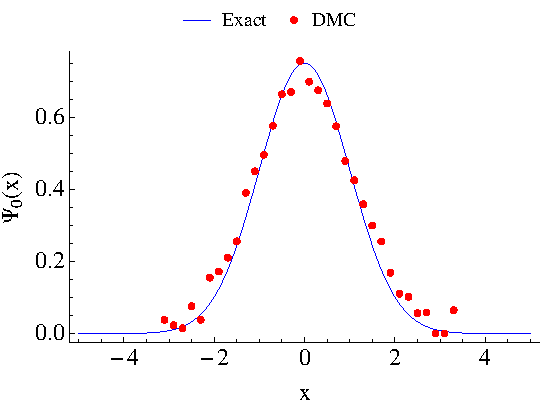
\includegraphics[width=0.5\textwidth]{notexact}
    \caption{DMC results for 1-d harmonic oscillator. Number of initial walkers was 10000, time step was 0.01, and number of time steps was 500. The exact energy is $E=\frac{1}{2}\hbar\omega$ and the DMC energy was $E=0.49\hbar\omega$.}
    \label{fig:1dho}
\end{figure}
I also did a calculation for a particle in a potential $V(x)=\frac{1}{2}x^4$, using the exact solution for the harmonic oscillator as the trial wave function. The DMC energy for this calculation was $E=0.57\hbar\omega$, and the resulting ground state wave function is shown in figure~\ref{fig:1dho4}.
\begin{figure}[h!]
  \centering
    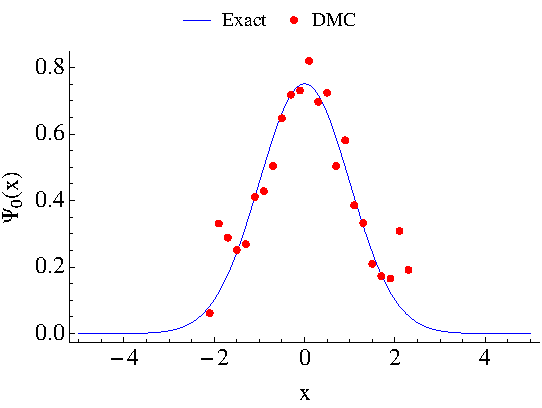
\includegraphics[width=0.5\textwidth]{notexact4}
    \caption{DMC results for particle in an $x^4$ potential. Number of initial walkers was 1000, time step was 0.01, and number of time steps was 500. The DMC energy was $E=0.57\hbar\omega$. The exact solution in this case represents the exact solution for the quantum harmonic oscillator.}
    \label{fig:1dho4}
\end{figure}


\section*{Auxiliary Field Diffusion Monte Carlo}
The methods described above are adequate for describing spin-independent potentials, but as described in \cite{schmidt1999} the number of spin-isospin states is 
\begin{equation}
  \frac{A!}{Z!(A-Z)!}2^A,
\end{equation}
where $A$ is the nucleons and $Z$ is the number of protons, which is exponential in the number of particles. The number of states to be sampled quickly becomes large. The AFDMC method is then used to simplify these methods.

My goal is to improve the trial function used in the current version of the code and so my comments will be directed toward this goal. The simplest trial wave function you can have is a slater determinant, which is the determinant of all of the single particle orbitals.
\begin{equation}
  \Psi_T(\mathbf{r}) \doteq \left| \\
  \begin{array}{cccc}
    \phi_1(\mathbf{r_1}) & \phi_2(\mathbf{r_1})  & \cdots & \phi_N(\mathbf{r_1})  \\
    \phi_1(\mathbf{r_2})  & \phi_2(\mathbf{r_2})  & \cdots & \phi_N(\mathbf{r_2})  \\
    \vdots & \vdots & \ddots & \vdots \\
    \phi_1(\mathbf{r_N})  & \phi_2(\mathbf{r_N})  & \cdots & \phi_N(\mathbf{r_N})  
  \end{array} \right|
\end{equation} 
This trial wave function does not include correlations. Ideally correlations would be included as
\begin{equation}
  \left<\mathrm{RS}\middle|\Psi_T\right> = \left<\mathrm{RS}\right| \prod\limits_{i<j}\left[f_c(r_{ij})\left[1+\sum\limits_{i<j,p}u_{ij}^p\mathcal{O}_{ij}^p\right]\right] \left|\Phi\right>,
  \label{equ:corrfull}
\end{equation}
where the sum on $p$ in our code goes from $1$ to $6$, where the first 6 $\mathcal{O}_{ij}^p$ are $1$, $\mathbf{\sigma}_i \cdot \mathbf{\sigma}_j$, $3\mathbf{\sigma}_i \cdot \hat{r}_{ij}\mathbf{\sigma}_j \cdot \hat{r}_{ij} - \mathbf{\sigma}_i \cdot \mathbf{\sigma}_j$, and the same things multiplied by $\mathbf{\tau}_i \cdot \mathbf{\tau}_j$. However, this requires too many operations. As discussed in \cite{gandolfi2014} the correlations have currently been included as
\begin{equation}
  \left<\mathrm{RS}\middle|\Psi_T\right> = \left<\mathrm{RS}\right| \left[\prod\limits_{i<j}f_c(r_{ij})\right]\left[1+\sum\limits_{i<j,p}u_{ij}^p\mathcal{O}_{ij}^p\right] \left|\Phi\right>.
  \label{equ:corrsimp}
\end{equation}
This is a first approximation and does not include many terms in the interaction. The next step to move from equation~\ref{equ:corrsimp} to equation~\ref{equ:corrfull} is to add the independent pair terms. This would look like
\begin{equation}
  \left<\mathrm{RS}\middle|\Psi_T\right> = \left<\mathrm{RS}\right| \left[\prod\limits_{i<j}f_c(r_{ij})\right]\left[1+\sum\limits_{i<j,p}u_{ij}^p\mathcal{O}_{ij}^p + \sum\limits_{i<j,p}\sum\limits_{k<l,p}u_{ij}^p\mathcal{O}_{ij}^pu_{kl}^p\mathcal{O}_{kl}^p\right] \left|\Phi\right>. 
\end{equation}
I am currently working on understanding the code so that I can add these extra terms into the trial wave function.

Even though my project does not deal with the sampling of the spin states I will mention the idea here for completeness. As discussed in \cite{schmidt1999} the non-central part of the potential can be written in the form
\begin{equation}
  V_\mathrm{nc} = \frac{1}{2} \sum\limits_{n=1}^{3N}(O_n^{(\sigma)})^2\lambda_n^{(\sigma)} + \frac{1}{2} \sum\limits_{\alpha=1}^{3} \sum\limits_{n=1}^{3N}(O_{n\alpha}^{(\sigma\tau)})^2\lambda_n^{(\sigma\tau)} + \frac{1}{2} \sum\limits_{\alpha=1}^{3} \sum\limits_{n=1}^{N}(O_{n\alpha}^{(\tau)})^2\lambda_n^{(\tau)},
\end{equation}
where the three squared operators are given by
\begin{equation}
  \begin{split}
    O_n^{(\sigma)} &= \sum\limits_i \boldsymbol{\sigma}_i \cdot \boldsymbol{\psi}_n^{(\tau)}(i) \\
    O_{n\alpha}^{(\sigma\tau)} &= \sum\limits_i \tau_{i\alpha} \boldsymbol{\sigma}_i \cdot \boldsymbol{\psi}_n^{(\sigma\tau)}(i) \\
    O_{n\alpha}^{(\tau)} &= \sum\limits_i \tau_{i\alpha} \psi_n^{(\tau)}(i),
  \end{split}
\end{equation}
where the $\psi$'s are the eigenfunctions of symmetric matrices that consist of phenomenological data. At this point the Hubbard-Stratonovich transformation can be used to take these squared operators and convert them to linear operators using the equation
\begin{equation}
  e^{-\frac{1}{2}\lambda_n O_n^2\Delta t} = \left( \frac{\Delta t |\lambda_n|}{2\pi} \right)^{1/2} \int\limits_{-\infty}^{\infty} dx e^{-\frac{1}{2}\Delta t |\lambda_n|x^2 - \Delta t s \lambda_n O_n x}.
\end{equation}
Notice how the $O_n$ term goes from quadratic to linear. This transformation is what gives the method the name Auxiliary Field.


\section{Conclusion and Outlook}
As mentioned before, one of the most important parts of the calculation is to have a good estimate for the trial wave function that is possible and inexpensive to calculate. So far we have implemented and tested a method for improving the trial wave function used in AFDMC calculation of nuclei and nuclear matter. We have done this by including independent pair and the full quadratic terms in the correlation operator which currently only has linear terms. The addition of these optimized terms has caused the energy of ${}^{4}$He, ${}^{16}$O and SNM to decrease.

Another way to improve the trial wave function is to include more terms in the expansion of the product correlation operator in Eq.~\ref{equ:prodpsi}. As we have learned from the independent pair expansion that we implemented, this would get computationally intractable as the number of particles gets large. Another alternative is to rewrite the correlation operator in terms of a Hubbard-Stratanovich transformation as is done with the spin-isospin dependent part of the propagator in Sec.~\ref{sec:AFDMC}. Future work will be done to handle the correlation operators in this way. We will also be searching for additional ways to improve the trial wave function.

With an improved trial wave function we will be using AFDMC to investigate some interesting aspects of nuclear physics and nuclear astrophysics. For example, we will be investigating the formation of deuteron and alpha particle clusters at various densities in mostly neutron matter. Many types of clustering in physics deal with two particles at a time. Alpha particles are thus a special case of four fermion clustering due to the two additional isospin degrees of freedom in addition to the two spin states for spin 1/2 particles. Work has been done to show the light clustering ($A\leq4$) and condensation of particles in nuclear systems, \cite{schuck2007,schuck2013_1,schuck2013_2} including neutron stars \cite{avancini2010,avancini2012,raduta2014}. We plan to show that the AFDMC method, with an improved nuclear wave function can be used to study properties of light clustering in nuclear systems as well. One way we will be doing this will be to do AFDMC calculation with 14 neutrons in a periodic box with the addition of 2 protons at a variety of densities to observe the formation of an alpha particle in neutron matter. Once these clusters are observed with AFDMC the density can be varied to determine the density at which the clusters dissolve as in Ref.\cite{avancini2012}. This work will be especially applicable to the study of alpha formation in neutron stars.

In conclusion, we have done AFDMC calculations to calculate the energy of ${}^4$He and ${}^{16}$O as well as the energy per particle of SNM. We have done these calculations with both linear correlation terms, linear plus independent pair correlations and linear plus all of the quadratic correlations in the trial wave function. In order to maintain the cluster decomposability of the trail wave function, which is lost with either the linear or independent pair correlations, we will be using the Hubbard-Stratanovich transformation to sample the exponential spin-isospin dependent correlations. This is analogous to the sampling of spin-isospin states in the propagator of AFDMC. We will also be looking for additional ways to improve the trial wave function. We will then be applying these calculations to other interesting nuclear systems such as the clustering of alpha particles in neutron matter.


\bibliographystyle{unsrt} % unsrt shows in order of citations
\bibliography{references.bib}

\end{document}
